%%
%% This is file `introduction.tex',
%%
The engineering standard for blast-resistant design is the Unified Facilities Criteria (UFC) 3-340-02 \cite{UFC3-340-02-2008}.  It is used extensively in the United States, United Kingdom, Australia, and Canada.   The primary blast-parameters used for protective design in the UFC are the:
\begin{itemize}
  \item incident-pressure,
  \item incident-impulse,
  \item reflected-pressure, and
  \item reflected-impulse.
\end{itemize}

The Kingery-Bulmash (KB) models are used to estimate these blast-parameters in the UFC.  The models are presented as a series of charts (free-air spherical and surface hemispherical) and are based on higher-order polynomials \cite{Kingery1984}.  The KB models are valid over a scaled distance of, $Z = 0.134 - 100$, where $Z=R/W^{1/3}$, $R$ is the distance from the center of the charge to the point of interest and $W$ is the charge weight (mass). At small scaled distances the KB models for incident impulse and positive phase duration show a local maximum, see Figures \ref{fig:KB_incident_impulse} and \ref{fig:KB_ppd}}.

\begin{figure}[tb]
  \begin{center}
   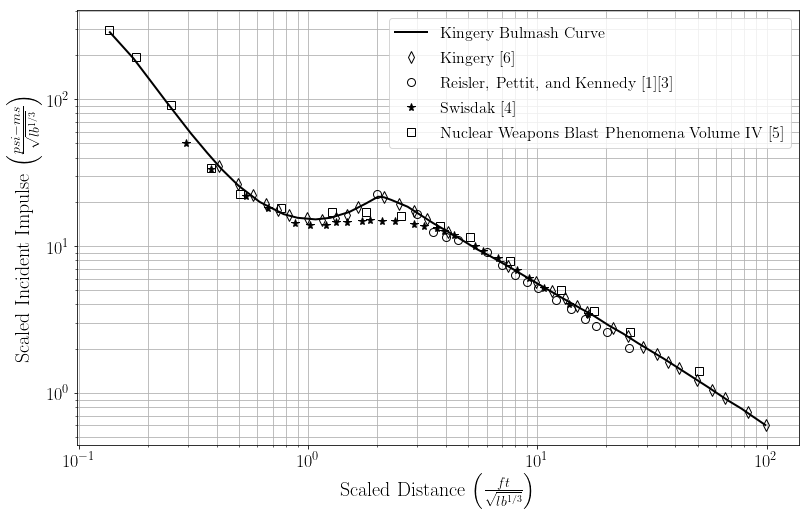
\includegraphics[width=6in]{/Users/skmcneill/Documents/Github/comprehensive/5_reports/figures/2018-12-19_kb_sii.png}
  \end{center}
  \caption{Kingery Bulmash incident impulse plot showing the inflection point forming at a scaled distance less than $5.00\: \nicefrac{ft}{\sqrt[3]{lb}}$\citep{Kingery1984}.}
\label{fig:KB_incident_impulse}
\end{figure}%
   
\begin{figure}[tb]
  \begin{center}
   \includegraphics[width=6in]{/Users/skmcneill/Documents/Github/comprehensive/5_reports/figures/2018-12-19_kb_ppd.png}
  \end{center}
  \caption{Kingery Bulmash postive phase duration plot showing the inflection point forming at a scaled distance less than $5.00\: \nicefrac{ft}{\sqrt[3]{lb}}$\citep{Kingery1984}.}
\label{fig:KB_ppd}
\end{figure}%


In the case of the scaled incident impulse, this local maximumThese inflection points result in an increase in the impulse loading that a structure must be able to withstand. Additionally, the KB positive phase duration data shows significant data scatter at small scaled distances.  calling into question the validity of the KB model at these .   Unfortunately, close-in blast loads represent a common threat for the protective design of buildings, bridges and critical infrastructure \cite{Shin2015a}\cite{Shin2014}.

It is hypothesized in this research, that the data scatter and the non-linear behavior of two of the KB models at small scaled distances is due to the presence of afterburn of the detonation reaction products.  The two KB models that show this non-linear behavior in the form of inflection points are the incident-impulse and the postive-phase-duration, see Figures \ref{fig:KB_incident_impulse} and \ref{fig:KB_TOA}. 
  

\section{Statement of the Problem}
Detonations at small scaled-distances represent a common threat to the blast-resistant design of buildings, bridges and critical infrastructure due to proximity in urban areas and lack of protection in rural locations. The Kingery-Bulmash curves used to predict the blasting loading show significant non-linear behavior (inflection points) at small scaled distances.  This non-linear behavior at small scaled distances is not well understood nor fully supported by empirical data.
In this research, we examine the influence of explosive oxygen-balance on the non-linear behavior observed in the Kingery-Bulmash curves. We record incident-overpressure, incident-impulse, time-of-arrival, positive-phase-duration, shock-velocity, fireball diameter, and fireball temperature for three different explosives with increasing oxygen balance in the air and three different explosives with increasing oxygen balance in neutral atmospheres.   Our objective is to determine the degree to which differences in explosive oxygen-balance on the measured blast parameters are causing the non-linear behavior observed.  Additionally, revised Kingery-Bulmash models of relevant blast parameters as a function of oxygen-balance will be developed based on the blast parameters measured during testing.

\section{Research and Scope Objectives}
The primary objective of this research is to quantify the effect explosive oxygen balance has on shockwave blast parameters at small scaled distances. This will lead to the secondary objective, the development of an improved Kingery Bulmash model that accounts for the oxygen balance of the explosive. The elements of these objectives include the following: 
\begin{itemize}
    \item determine the near field positive-phase-duration, incident impulse, and other relevant blast parameters of explosives with a range of oxygen balances,
    \item evaluate fireball diameter and temperature for explosives with a range of oxygen-balances.
    \item validate the influence of oxygen balance by detonating the same range of explosives in inert atmospheres, and
    \item develop a modified Kingery Bulmash model that accounts for oxygen balance.
\end{itemize}
 
\section{Originality of PhD Research}
This research is novel in hypothesizing a cause for the inflection point observed in the near field Kingery Bulmash model. Currently, there is no clear and concise explanation for this effect. This research would aid in the design of blast resistant structures by providing a more accurate model. This would in turn lead to an increased survivability in a structure.
\section{Research Methodology}
This research will empirically determine the near positive-phase-duration and incident-impulse of the following explosives:
\begin{itemize}
    \item trinitrotoluene (oxygen balance: -74\%),
    \item PETN (oxygen balance: -10\%)
    \item Dyno AP (oxygen balance: 0\%).
\end{itemize}
Pressure transducers will measure the time of arrival, incident impulse, and other blast parameters.  The explosives will be hemispherical in shape to minimize near-field shape effects.  The explosive charge will centered on a horizontal steel plate with incident pressure gauges positioned along a single axis.  Regression analysis will be used to describe the relationship between scaled distance, oxygen balance, and blast parameter data.

Simultaneous with the blast-parameter measurements, the fireball diameter and fireball temperature will be measured with a high-speed camera and spectrometer respectively.  Regression analysis will be used to determine a relationship between the measured blast parameters and the fireball diameter and temperature.

A set of validation experiments will be conducted using the same explosives and incident pressure gauge configuration, but placed in inert helium atmosphere.  If the hypothesis is correct, the oxygen balance of the explosives should not influence the positive phase duration or the incident impulse.

Finally, the Kingery Bulmash model will be modified to account for the explosive oxygen balance.
\section{Expected Contributions}
The expected contributions of this research are as follows:
\begin{itemize}
    \item development of improved Kingery-Bulmash models that account for the explosive oxygen-balance at small scaled distances,
    \item empirical evidence of blast parameters in the near field, and
    \item improved blast loading calculations for blast resistant designs.
\end{itemize}
\section{Academic Background Preparation of Candidate}
S. Kevin McNeill is currently a graduate student pursuing a Doctor of Philosophy in Explosive Engineering at Missouri University of Science and Technology (MST). H	e holds a Bachelors of Science in Mechanical Engineering from Louisiana State University and a Masters of Science in Explosive Engineering from MST. He is currently the Chief, of the Explosives Research and Development Division at the Bureau of Alcohol, Tobacco, Firearms, and Explosives (ATF).  In this position, he has conducted numerous government studies involving the measurement of overpressure and other blast parameters for the National Counter Terrorism Center, U.S. Army Corps of Engineers, Department of Defense Explosives Safety Board, and the Joint Improvised Explosive Device Agency.  In these studies, he has conducted test preparation, instrumentation selection, range layout, test controls, firing train selection, data analysis, and report writing.
%%
%% End of file `introduction.tex'.
